\subsection{UC-12}
\label{subsec:UC-12}

\begin{figure}[H]
    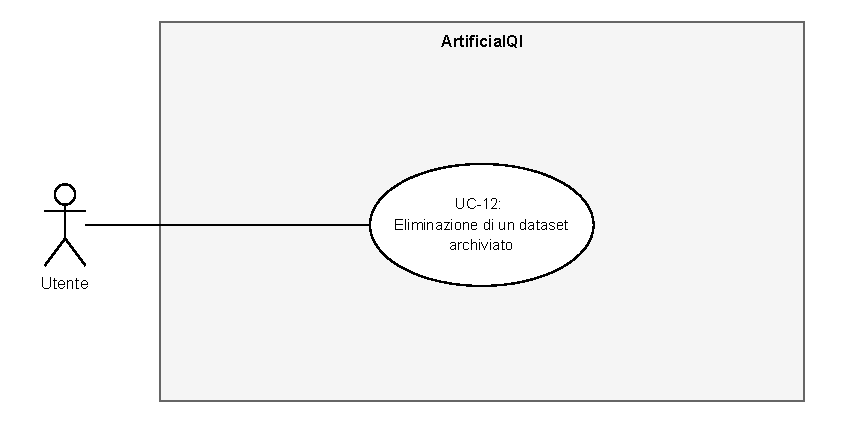
\includegraphics{Sezioni/UseCase/Immagini/UC-12.pdf}
    \caption{Diagramma UC-12.}
\end{figure}

\begin{usecase}{UC-12}{Eliminazione di un dataset archiviato}

    \req{\hyperref[item:RU-3]{RU-3}} 

    \pre{
        \item Il sistema è attivo e funzionante
        \item Il dataset archiviato da eliminare esiste
    }

    \post{
        \item Il dataset selezionato viene eliminato 
    }
    
    \actor{Utente}

    \subactors{}

    \trigger{L'utente deve eliminare un dataset archiviato}
    
    \inc{}

    \base{}

    \scenario{
        \item L'utente richiede l'eliminazione di un dataset archiviato
        \item L'utente conferma l'eliminazione del dataset selezionato
        \item Il dataset viene eliminato dal sistema
    }

    \subscenario{
        \item[2.1] \textbf{L'utente annulla l'eliminazione del dataset selezionato}
        \begin{itemize}
            \item[a.] Il dataset selezionato non viene eliminato
            \item[b.] Viene interrotta l'operazione di eliminazione
        \end{itemize}
        \item[3.1] \textbf{L'eliminazione del dataset dal sistema produce un errore}
        \begin{itemize}
        \item[a.] Viene notificato all'utente l'errore che ha impedito la corretta eliminazione del dataset selezionato
        \end{itemize}
    }

\end{usecase}